\documentclass[a4paper,11pt]{article}

% Macht evtl unter Windows Probleme?
\usepackage[utf8]{inputenc}

% weitere Pakete hier
\usepackage{amsmath}
\usepackage{graphicx}
\usepackage{multicol}
\usepackage{xcolor}

\definecolor{comment_color}{RGB}{63,127,89}
\definecolor{keyword_color}{RGB}{127,0,85}
\definecolor{string_color}{RGB}{42,0,255}
\usepackage{listings}
\lstset{language=Java,
  basicstyle=\ttfamily,
  commentstyle=\color{comment_color},
  keywordstyle=\color{keyword_color},
  showstringspaces=false,
  stringstyle=\color{string_color},
}

% Referenzen schön formatieren, Kommandos
% \cite  -> [x]
% \citet -> Name [x]
\usepackage[sort&compress,numbers]{natbib}
\setlength{\bibsep}{2pt plus 0.3ex}
\renewcommand*{\bibfont}{\small}
\makeatletter
\def\NAT@spacechar{~}% NEW
\makeatother

% Klickbare Links im Dokument
\usepackage{hyperref} % muss als vorletztes Paket eingebunden werden
% Evtl auskommentieren

% Querverweise mit \cref und \Cref
\usepackage[ngerman]{babel}
\usepackage[ngerman,noabbrev]{cleveref} % muss als letztes Paket eingebunden werden


%%%%%%%%%%%%%%%%%%%%%%%%%%%%%%%%%%%%%%%%
\title{\textbf{EvoSuite}\\
Automatisierte Generierung von Testsuiten für Java}
\author{Adrian Uffmann\\
Matrikelnummer: 12043921\\
\texttt{adrian.uffmann@campus.lmu.de}}
\date{09.02.2020}
%%%%%%%%%%%%%%%%%%%%%%%%%%%%%%%%%%%%%%%%

\begin{document}
\maketitle

\begin{center}
Masterseminar Fuzz Testing
\end{center}

\begin{abstract}
EvoSuite ist ein Programm, welches mithilfe eines genetischen Algorithmus automatisiert JUnit-Testfälle aus Java-Bytecode generieren kann.
Diese Seminararbeit gibt einen Überblick über die Funktionsweise von EvoSuite und fasst die Ergebnisse einer empirischen Studie über die Praxistauglichkeit dieses Werkzeugs zusammen.
Insbesondere wird dabei klar, dass mehr Forschungsbedarf besteht, um die Errungenschaften im Bereich von \textit{Search-Based Software Testing} auch in der professionellen Softwareentwicklung nutzen zu können.
\end{abstract}

\section{Einleitung}

Das Testen von Software ist ein wichtiger Teil der Softwareentwicklung.
So schreiben \citet{myers2004art}:
\begin{quote}
it [is] a well-known rule of thumb that in a typical programming project approximately 50 percent of the elapsed time and more than 50 percent of the total cost [are] expended in testing the program or system being developed.
\end{quote}
Daher ist es kaum verwunderlich, dass es zahlreiche Werkzeuge gibt, die helfen sollen, das Testen von Software zu automatisieren.
EvoSuite geht noch einen Schritt weiter: hier wird nicht versucht das Testen der Software zu automatisieren, sondern das Erstellen von automatisierten Tests selbst durch Automatisierung zu vereinfachen.
Der Fokus liegt dabei auf der Optimierung eines \textit{test last} Ansatzes, d.~h. getestet wird erst, nachdem das eigentliche Programm fertig implementiert ist.
Bei diesem Ansatz würde sich ein Softwaretester zunächst Szenarien überlegen, mit denen er möglichst viele Pfade des Programms abdeckt und diese als Unittests ausformuliert.
Mithilfe von sogenannten Orakeln wird dabei ein bestimmtes Verhalten des Programms definiert.
Verhält sich das Programm anders als von den Orakeln vorgegeben, so schlägt der Test fehl und es wurde ein Bug gefunden.

EvoSuite versucht nun diesen Prozess zu vereinfachen, indem es Unittests generiert, die das Verhalten des Programms möglichst gut beschreiben.
Ein Softwaretester muss sich dann nicht mehr selbst Szenarien überlegen, sondern nur noch die generierten Testfälle auf unerwartetes Verhalten prüfen.
Dazu nutzt EvoSuite einen genetischen Algorithmus, mit dem zufällige Test-fälle immer weiter verbessert werden, bis sie eine möglichst hohe Testabdeckung erreichen.
Die Testfälle werden dann minimiert, um die Arbeit des Softwaretesters zu vereinfachen und es werden mit sogenanntem \textit{Mutation-Testing} möglichst repräsentative Orakel ausgewählt.

EvoSuite wurde seit 2010 immer weiter entwickelt und es sind verschiedene Algorithmen für das Generieren von Testfällen implementiert, die über die Kommandozeile ein- und ausgeschaltet werden können.
Dazu haben die Autoren von EvoSuite auf der Internetseite (\url{http://www.evosuite.org/publications}) 54 Artikel über die Konzepte in und die Evaluation von EvoSuite und dessen Vorgänger ${\mu}Test$ veröffentlicht.
Um den vorgegebenen Umfang einzuhalten, kann diese Seminararbeit nur Überblick über einen kleinen Teil von EvoSuite geben.

\section{Genetische Algorithmen}
\label{sec:genetische_algorithmen}

Genetische Algorithmen gehören zu den evolutionären Algorithmen.
Die Idee dabei ist es, den Prozess der Evolution und natürlichen Auslese aus der Biologie zu simulieren, um Optimierungsprobleme zu lösen.
Dazu werden Lösungskandidaten für das Optimierungsproblem als Individuen betrachtet.
Die Menge der betrachteten Individuen nennt man auch Population oder Generation.

Ausgehend von einer Anfangspopulation werden mit einer bestimmten Wahrscheinlichkeit durch Rekombination und Mutation neue Individuen erzeugt.
Bei einer Rekombination werden aus mehreren Eltern-Individuen ein oder mehrere neue Kind-Individuen erzeugt, während bei einer Mutation aus nur einem Individuum durch eine kleine Änderung ein neues Individuum entsteht.
Die neuen Individuen werden anhand einer Fitnessfunktion bewertet und anhand von dieser Bewertung wird eine Menge der Individuen ausgewählt, um die neue Population zu bilden.
Die restlichen Individuen werden verworfen.

Dieser iterative Prozess wird so lange ausgeführt, bis entweder ein Individuum gefunden wurde, welches das Optimierungsproblem optimal löst, bis eine vorgegebene Anzahl an Generationen entwickelt wurde oder bis die verfügbare Zeit aufgebraucht ist.
In jedem Fall ist das Ergebnis des genetischen Algorithmus das beste Individuum.

Um ein konkretes Optimierungsproblem mit einem genetischen Algorithmus zu lösen, muss genau definiert werden, was ein Individuum ist, aus welchen Individuen die Anfangspopulation besteht, wie die Rekombinations- und Mutationsoperatoren neue Individuen erzeugen und wie die Fitnessfunktion aussieht.
Dies ist von Problem zu Problem unterschiedlich.

\section{Erzeugen von Testsuiten}
\label{sec:erzeugen_von_testsuiten}

\subsection{Betrachten von Testsuiten in ihrer Gesamtheit}

EvoSuite beginnt mit dem Generieren von Testfällen ohne Orakel.
Dafür werden verschiedene Algorithmen angeboten.
In dieser Seminararbeit wird jedoch nur das Verbessern von ganzen Testsuiten hinsichtlich der Testabdeckung mit einem genetischen Algorithmus nach \cite{TSE12_EvoSuite} beschrieben.

Die Verbesserung von Testsuiten in ihrer Gesamtheit ist dabei eine wichtige Neuerung, die vor EvoSuite, nach bestem Wissen der Autoren, nicht verwendet wurde.
Nach \cite{TSE12_EvoSuite} betrachteten die meisten anderen Werkzeuge nur einzelne Programmpfade sequenziell und versuchten Testfälle zu generieren, die diese ausgewählten Pfade abdeckten.
Ein großes Problem bei diesem Ansatz ist jedoch, dass nicht jeder Programmpfad auch erreichbar ist.
Wenn versucht wird, einen unerreichbaren Pfad zu erreichen, dann ist der dafür verwendete Aufwand verschwendet.
Ob ein bestimmter Pfad überhaupt erreichbar ist, ist allerdings ein unentscheidbares Problem, da man sonst das Halteproblem lösen könnte.
Bei diesem Ansatz ist es demnach sehr wichtig, mit welchen Programmpfaden begonnen wird.

Ein weiterer Nachteil ist kollaterale Abdeckung.
Dieses Problem kann auftreten, wenn zunächst Testfälle generiert werden, die einfache Pfade nahe der Oberfläche des Programms abdecken.
In diesem Fall werden dieselben Pfade auch erreicht, wenn später Testfälle für tiefere Pfade des Programms generiert werden.
Dadurch werden die zuerst generierten Testfälle nutzlos, da sie keinen Beitrag mehr zur Testabdeckung leisten und der Aufwand, sie zu generieren, war verschwendet.

EvoSuite vermeidet diese Probleme, indem die Testabdeckung der gesamten Testsuite auf einmal verbessert wird.
Statt einzelne Programmpfade auszuwählen, die erreicht werden sollen, wird bei EvoSuite gemessen, wie weit die gesamte Testsuite davon entfernt ist, alle Programmpfade abzudecken.

\subsection{Testsuiten als Individuen}

Wie in \cref{sec:genetische_algorithmen} erwähnt, muss für die Nutzung eines genetischen Algorithmus zunächst definiert werden, wie ein Individuum aussieht.
Da EvoSuite ganze Testsuiten auf einmal betrachtet, ist ein Individuum eine Testsuite.
Eine Testsuite ist dabei eine Menge von Testfällen ($T = \{t_1, t_2, ..., t_n\}$), wobei ein Testfall eine Sequenz von Anweisungen ist ($t = \langle s_1, s_2, ..., s_l \rangle$).
In EvoSuite wird zwischen 5 Arten von Anweisungen unterschieden:
\begin{itemize}
	\item Primitive Anweisungen, wie \lstinline{int var0 = 54},\\
	oder \lstinline{Object[] var1 = new Object[10]}.
	\item Zuweisungen, wie \lstinline{var1[0] = new Object()},\\
	oder \lstinline{var2.maxSize = 10}.
	\item Feld-Anweisungen, wie \lstinline{int var3 = var2.size}.
	\item Konstruktor-Anweisungen, wie \lstinline{Stack var2 = new Stack()}.
	\item Methoden-Anweisungen, wie \lstinline{int var4 = var2.pop()}.
\end{itemize}
Der Sprachumfang von Java erlaubt deutlich mehr Arten von Anweisungen, wie z.~B. \lstinline{if}-Anweisungen, \lstinline{while}- und \lstinline{for}-Schleifen.
Diese sind jedoch nicht in Testfällen erwünscht, da Testfälle deterministisch sein sollen und keine Parameter erhalten, die sich auf den Kontrollfluss auswirken könnten.
Außerdem enthalten die hier definierten Testfälle keine Orakel, wie z.~B. \textit{Assertions}.
Diese werden in einem späteren Schritt hinzugefügt (Siehe \cref{sec:erzeugen_von_orakeln}).

Für den noch zu definierenden Mutationsoperator ist es wichtig festzuhalten, dass jede Anweisung einen Wert von einem bestimmten Typ bereitstellt, der in späteren Anweisungen verwendet werden kann.
Für eine Anweisung $s$ wird dieser Wert im folgenden als $v(s)$ bezeichnet.

\subsection{Erzeugen neuer Individuen}

Als Nächstes müssen die Rekombination und Mutation definiert werden.
Diese beiden Operatoren sind in \cref{fig:rekombination_und_mutation} schematisch dargestellt.

Die Rekombination ist in EvoSuite sehr einfach gehalten.
Hierbei werden mit einer bestimmten Wahrscheinlichkeit aus den beiden Eltern-Testsuiten $P_1$ und $P_2$ die beiden Kind-Testsuiten $O_1$ und $O_2$ erstellt.
Zunächst wird ein Anteil $\alpha \in [0;1]$ gewählt.
Das Kind $O_1$ ergibt sich, indem der Anteil $\alpha$ der Testfälle von $P_1$ mit einem Anteil $(1 - \alpha)$ der Testfälle von $P_2$ kombiniert wird.
Das Kind $O_2$ besteht dann aus den übrigen $(1 - \alpha) \times |P_1|$ Testfällen von $P_1$ und den übrigen $\alpha \times |P_2|$ Testfällen von $P_2$.
Individuen können durch diese Rekombination nicht länger oder kürzer werden, als der längste, bzw. kürzeste Elternteil.
Im Durchschnitt nähern sich dadurch alle Individuen der gleichen Anzahl an Testfällen an.

\begin{figure}
	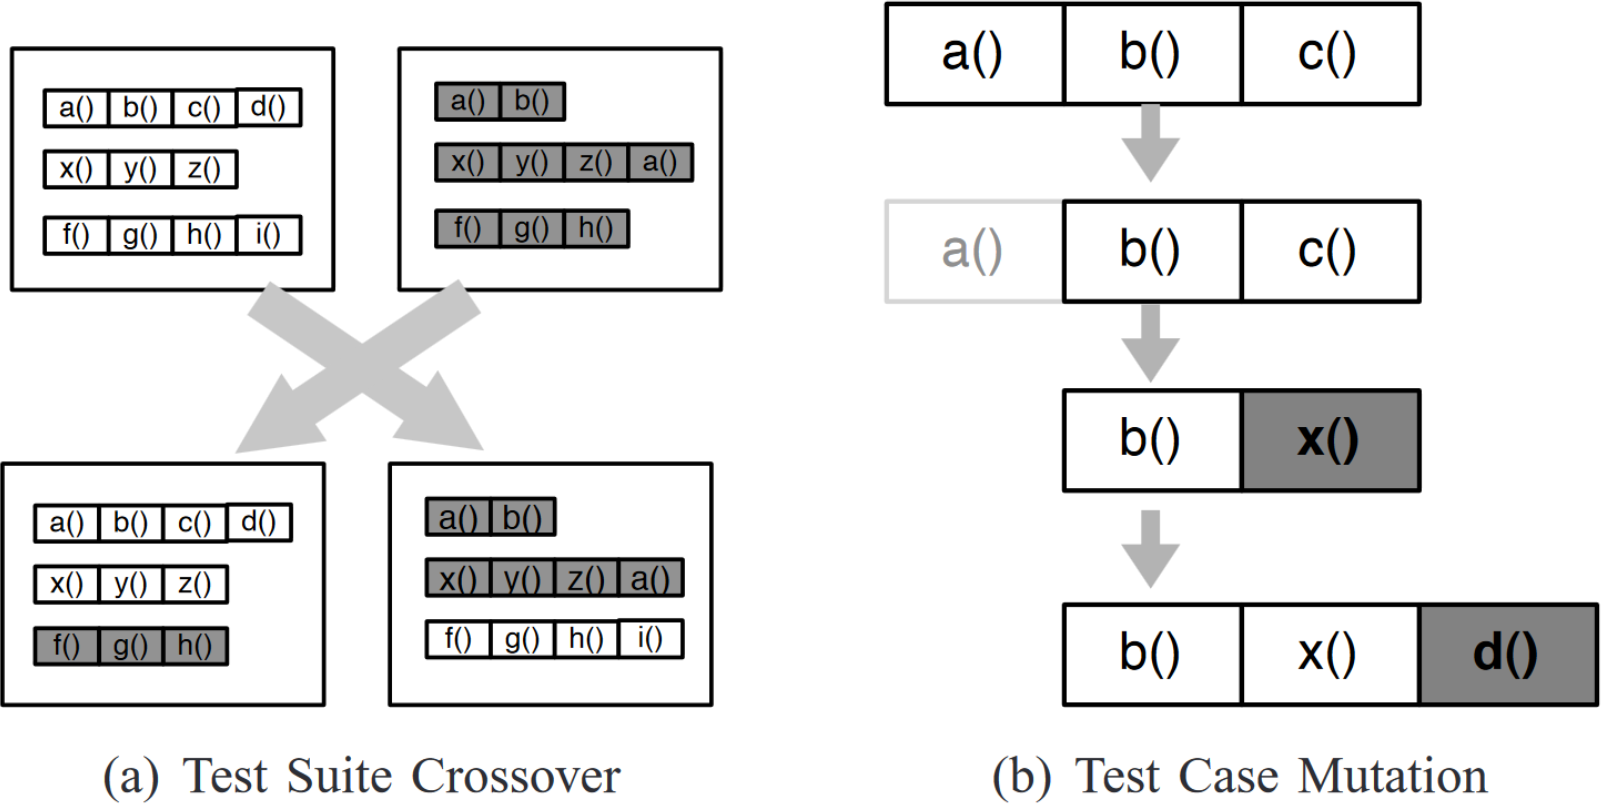
\includegraphics[width=\textwidth]{evosuite-crossover-and-mutation.png}
	\caption{Rekombination und Mutation aus \citep{TSE12_EvoSuite}}
	\label{fig:rekombination_und_mutation}
\end{figure}

Die Mutation einer Testsuite $T$ ist deutlich komplexer, als die Rekombination.
Hierbei wird jeder Testfall $t$ mit einer Wahrscheinlichkeit von $\frac{1}{|T|}$ mutiert.
Im Durchschnitt wird bei der Mutation einer Testsuite also genau ein Testfall mutiert.
Es ist aber auch möglich, dass keiner oder mehrere Testfälle auf einmal mutiert werden. Bei der Mutation eines Testfalls werden der Reihe nach folgende Operationen jeweils mit einer Wahrscheinlichkeit von $\frac{1}{3}$ durchgeführt:
\begin{enumerate}
	\item Entfernen von Anweisungen.
	\item Ändern von Anweisungen.
	\item Einfügen von Anweisungen.
\end{enumerate}

Beim Entfernen von Anweisungen wird jede Anweisung $s_i$ mit einer Wahrscheinlichkeit von $\frac{1}{|t|}$ entfernt.
Da der Wert $v(s_i)$ in einer späteren Anweisung benutzt werden könnte, müssen alle Anweisungen $\{s_j \in t | j > i\}$ überprüft werden, um sicherzustellen, dass ein valides Individuum entsteht.
Wenn ein $s_j$ den Wert $v(s_i)$ verwendet, dann wird dieser durch einen anderen verfügbaren Wert desselben Typs ersetzt.
Wenn in dem Testfall keine andere Anweisung einen Wert mit demselben Typ bereitstellt, dann wird $s_j$ rekursiv entfernt.
Bleibt nach dem Entfernen von Anweisungen ein leerer Testfall übrig, dann wird dieser komplett gelöscht.

Beim Ändern von Anweisungen wird wieder jede Anweisung mit einer Wahrscheinlichkeit von $\frac{1}{|t|}$ geändert.
Hier werden verschiedene Arten von Anweisungen verschieden behandelt.

Bei primitiven Anweisungen wird einfach der primitive Wert um einen zufälligen $\Delta$-Wert erhöht oder erniedrigt, Arrays werden verlängert oder verkürzt und Zeichenketten werden mutiert.
Bei der Verkürzung von Arrays muss genau wie beim Entfernen von Anweisungen darauf geachtet werden, dass spätere Anweisungen keine entfallenen Arrayindizes verwenden.
Die Mutation von Zeichenketten funktioniert ähnlich, wie die Mutation von Testfällen.
Es werden neue Zeichen eingefügt, bestehende Zeichen geändert und alte Zeichen entfernt.

Bei Zuweisungen wird zufällig eine der beiden Seiten durch ein anderes Feld, bzw. einen anderen Wert ersetzt.

Für Feld-, Konstruktor- und Methoden-Anweisungen wird zufällig ein anderes Feld, ein anderer Konstruktor oder eine andere Methode ausgesucht, deren Parameter mit den verfügbaren Werten erfüllt werden können.
Dabei ist es z.~B. auch möglich, dass aus einer Feld-Anweisung eine Methoden-Anweisung wird.

Beim Einfügen von Anweisungen wird dem Testfall mit einer Wahrscheinlichkeit von $\sigma$ eine zufällige Anweisung hinzugefügt.
Als Parameter für Methoden- oder Konstruktoraufrufe werden dabei die bereitgestellten Werte wiederverwendet oder neue Werte generiert, die direkt eingesetzt werden.
Dies wird wiederholt, bis in einem Schritt mit einer Wahrscheinlichkeit von $(1 - \sigma)$ keine neue Anweisung eingefügt wird.
Durch dieses Vorgehen sinkt die Wahrscheinlichkeit weitere Anweisungen einzufügen exponentiell.
$i$ oder mehr Anweisungen werden also nur mit einer Wahrscheinlichkeit von $\sigma^i$ eingefügt.

Mit dem bis hier beschriebenen Mutationsoperator können Testfälle län-ger werden, kürzer werden oder sogar entfallen.
Es ist aber bisher nicht möglich, dass neue Testfälle entstehen und auch durch die Rekombination kann die Anzahl der Testfälle in einer Testsuite nicht größer werden, als die Anzahl der Testfälle im größeren Elternteil.
Aus diesem Grund wird bei der Mutation einer Testsuite nach dem Mutieren der Testfälle mit einer Wahrscheinlichkeit von $\sigma'$ ein zufälliger neuer Testfall erzeugt.
Genau wie bei dem Einfügen von Anweisungen werden hier mit exponentiell sinkender Wahrscheinlichkeit weitere Testfälle hinzugefügt.

Um einen Testfall zu erzeugen, wird eine zufällige Länge $l \sim [1, L]$ gewählt (wobei $L$ die maximal zugelassene Länge von Testfällen ist) und es werden so lange neue Anweisungen, wie bei der Mutation von Testfällen, eingefügt, bis der neue Testfall die gewünschte Länge erreicht hat.

Nun da die Mutation von Testsuiten definiert ist, ist es leicht, die Anfangspopulation zu definieren.
Als Anfangspopulation wird eine vorgegebene Anzahl an Testsuiten erzeugt, indem jede mit einer vorgegebenen Anzahl an zufälligen Testfällen befüllt wird.
Die zufälligen Testfälle werden dabei genau wie bei der Mutation von Testsuiten erstellt.

\subsection{Fitnessfunktion}

Als letztes muss für den genetischen Algorithmus noch die Fitnessfunktion definiert werden.
Hier implementiert EvoSuite verschiedene Ansätze.
Z.~B. können Testfälle mit \textit{Mutation-Testing} generiert werden \cite{emse14_mutation}.
In dieser Arbeit wird jedoch die Maximierung der Testabdeckung aus \cite{TSE12_EvoSuite} betrachtet.
Gesucht ist dabei eine Testsuite, die mit möglichst wenig Anweisungen möglichst viele Zweige der getesteten Klasse ausführt.
Jede Methode hat dabei einen Programmpfad (den Körper der Methode), welcher sich an einer \lstinline{if}-Anweisung in zwei Pfade aufteilt.
Diese Pfade können sich selbst wieder aufteilen oder wieder zu einem Pfad zusammenlaufen.
Da EvoSuite nicht Quellcode, sondern Bytecode betrachtet, sind kompliziertere Anweisungen, wie \lstinline{switch}-Anweisungen oder Schleifen bereits in einfache Verzweigungen übersetzt worden.
Eine optimale Testsuite führt demnach jede Anweisung in der getesteten Klasse aus, indem jede Bedingung mindestens einmal zu wahr und falsch evaluiert wird.

Da genetische Algorithmen durch Mutation nur kleine zufällige Änder-ungen erzeugen, ist es wichtig, dass bereits kleine Änderungen eine Verbesserung der Fitness erreichen können.
Wenn sich die Fitnessfunktion nur verbessert, wenn mehr Programmpfade abgedeckt werden, ist es sehr unwahrscheinlich, dass eine kleine Änderung die Fitness verbessert, da es sehr schwer ist, genau die richtigen Werte zu erraten, um eine Bedingung zu erfüllen.
Aus diesem Grund wird die \textit{branch distance} $d_{min}(b, T)$ von \citet{10.1109/32.57624} verwendet.

\begin{figure}[h]
	\begin{lstlisting}[basicstyle=\ttfamily\tiny]
public static int fakultaet(int n) {
  if (n > 16) { // Zweig b
    throw new IllegalArgumentException(n + "! is out of int range");
  }
  ...
}
	\end{lstlisting}
	\begin{multicols}{2}
		\begin{lstlisting}[basicstyle=\ttfamily\tiny]
@Test(timeout = 4000)
public void test01() throws Throwable {
  int int0 = fakultaet(1);
  assertEquals(1, int0);
}
		\end{lstlisting}
		\textit{branch distance} $\approx$ 16
		\columnbreak
		\begin{lstlisting}[basicstyle=\ttfamily\tiny]
@Test(timeout = 4000)
public void test10() throws Throwable {
  int int0 = fakultaet(10);
  assertEquals(3628800, int0);
}
		\end{lstlisting}
		\textit{branch distance} $\approx$ 7
	\end{multicols}
	\caption{Beispiel für \textit{branch distance}}
	\label{fig:branch_distance}
\end{figure}

Die Idee hierbei ist, dass eine Ausführung einer Bedingung besser ist, wenn die Variablen der Bedingung weniger geändert werden müssen, um sie zu erfüllen.
\cref{fig:branch_distance} zeigt ein Beispiel, wie die \textit{branch distance} für einen Zweig \texttt{b} vom Wert einer Variable \texttt{n} abhängt.
Wenn die Variable \texttt{n} den Wert 1 hat, muss sie noch um 16 geändert werden, um die Bedingung zu erfüllen.
Wenn die Variable \texttt{n} den Wert 10 hat, muss sie nur noch um 7 geändert werden.
Demnach ist der rechte Testfall näher am Ziel, Zweig \texttt{b} abzudecken.
Die \textit{branch distance} einer Testsuite ist einfach das Minimum der \textit{branch distances} der einzelnen Testfälle.

Tatsächlich ist die Berechnung der \textit{branch distance} etwas komplizierter, so wird z.~B. bei Bedingungen, die zu wahr evaluieren sollen, noch eine Konstante $k > 0$ addiert, es müssen auch komplexe Bedingungen mit mehreren Variablen berücksichtigt werden und manche Bedingungen werden wegen Verschachtelung gar nicht ausgeführt, bevor andere Bedingungen erfolgreich sind.
Um die Fitnessfunktion von EvoSuite zu verstehen sind diese Details aber nicht wichtig.

Eine optimale Testsuite $T$ soll also die Menge aller Methoden der getesteten Klasse $M$ ausführen und in den Methoden die Menge aller Zweige $B$.
Damit ergibt sich die zu minimierende Fitnessfunktion in \cref{fig:fitnessfunktion}.
$M_T$ ist dabei die Menge der Methoden der getesteten Klasse, die durch die Testsuite abgedeckt werden und die Funktion $v(x)$ ist eine Normalisierungsfunktion, um die \textit{branch distance} in einen Wertebereich von 0 bis 1 zu übersetzen.

\begin{figure}[h]
	$fitness(T) = |M| - |M_T| + \sum\limits_{b \in B} d(b, T)$

	$d(b, T) = \begin{cases}
	0 & \text{if the branch b has been covered,}\\
	v(d_{min}(b, T)) & \text{if the predicate was executed at least twice,}\\
	1 & \text{otherwise.}
	\end{cases}$

	$v(x) = \frac{x}{(x+1)}$
	\caption{Fitnessfunktion aus \cite{TSE12_EvoSuite}}
	\label{fig:fitnessfunktion}
\end{figure}

Wie man sieht, wird die \textit{branch distance} $d_{min}(b, T)$ von \citet{10.1109/32.57624} nur für Zweige verwendet, die mindestens zweimal ausgeführt werden.
Der Grund dafür ist, dass es für jede Bedingung zwei Zweige gibt.
Wenn eine Bedingung durch eine Testsuite nur einmal ausgeführt wird, ist die \textit{branch distance} nur für einen der beiden Zweige 0.
Eine Minimierung der \textit{branch distance} für den anderen Zweig würde aber dazu führen, dass der erste Zweig nicht mehr abgedeckt wird, da die Bedingung bei nur einer Ausführung nicht wahr und falsch sein kann.
Nun würde die Fitnessfunktion wiederum Individuen bevorzugen, die die \textit{branch distance} des ersten Zweigs minimieren und es ergibt sich ein oszillierendes Verhalten.
Dieses Problem wird durch die Fallunterscheidung in der Funktion $d(b, T)$ vollständig vermieden.

\section{Erzeugen von Orakeln}
\label{sec:erzeugen_von_orakeln}

Mit dem Vorgehen in \cref{sec:erzeugen_von_testsuiten} können Testsuiten mit möglichst hoher Testabdeckung erzeugt werden, aber diese Testsuiten enthalten noch keine Orakel.
Orakel werden in EvoSuite in einem zweiten Schritt generiert.
Dadurch kann der Algorithmus für das Erzeugen von Testfällen leicht angepasst oder ersetzt werden, ohne dass sich das auf das Erzeugen von Orakeln auswirkt.

EvoSuite nutzt für das Erzeugen von Orakeln sogenanntes \textit{Mutation-Testing} \cite{TSE12_Mutation, emse14_mutation}.
Die Idee dabei ist, das zu testende Programm durch kleine Mutationen zu verändern, um zu sehen, welche Orakel diese Änderung bemerken würden.
Mutation bedeutet hier etwas anderes als in den genetischen Algorithmen aus \cref{sec:genetische_algorithmen}.
Hier sind Mutationen kleine Änderungen, die typische Programmierfehler darstellen sollen.
Das kann zum Beispiel das Austauschen von arithmetischen Operationen oder das Entfernen von Methodenaufrufen sein.
Die vollständige Liste dieser Mutationsoperatoren befindet sich in \cite{emse14_mutation}.

Jedes mutierte Programm wird mit dem Originalprogramm verglichen und alle Orakel, die einen Unterschied zwischen den beiden feststellen, werden mit dem Mutanten assoziiert.
Man spricht hier auch davon, dass das Orakel den Mutanten tötet.
Als Orakel dienen in EvoSuite \textit{Assertions}.
Nach \citep{TSE12_Mutation} werden hier sieben Arten von \textit{Assertions} unterschieden:
\begin{itemize}
	\item Primitive Assertions, wie \lstinline{assertEquals(0, int0)}.
	\item Vergleichs-Assertions, wie \lstinline{assertFalse(var2.equals(var0))}.
	\item Inspektor-Assertions, wie \lstinline{assertEquals(0, intStack0.size())}.
	\item Feld-Assertions, wie \lstinline{assertEquals(1, intStack0.size)}.
	\item String-Assertions, wie \lstinline{assertEquals("P7W", var1.toString())}.
	\item Null-Assertions, wie \lstinline{assertNull(intStack1)}.
	\item Exception-Assertions.
\end{itemize}
Nachdem alle Mutanten betrachtet wurden, werden überflüssige \textit{Assertions} entfernt.
Das Ziel dabei ist es, so wenig \textit{Assertions} wie möglich zu behalten und trotzdem alle Mutanten zu töten.
Dieses Problem ist eine Instanz des NP-vollständigen \textit{minimum set cover} Problems.
Daher wird eine einfache Heuristik aus \cite{chvatal1979greedy} verwendet, bei der immer die \textit{Assertion} aufgenommen wird, die die meisten zusätzlichen Mutanten tötet, bis die Menge der aufgenommenen \textit{Assertions} alle Mutanten tötet.

\section{Evaluation}

EvoSuite wird öffentlich auf GitHub gehostet, wodurch der Quellcode einfach mit Git heruntergeladen werden konnte.
Mit einer Maven 3.6.2 Installation (\url{https://maven.apache.org}) konnte ich leicht eigene Versionen von EvoSuite basierend auf dem \textit{master-Branch} und \textit{1.0.6-Tag} bauen.
Leider schlugen einige Tests im \textit{evosuite-client}-Projekt fehl, daher musste ich Maven mit \texttt{mvn install -DskipTests} aufrufen.

Da EvoSuite Testfälle generiert, die von einem Tester evaluiert werden müssen, um Fehler zu finden, wäre es für diese Seminararbeit zu aufwändig EvoSuite an einer echten Bibliothek zu evaluieren.
Stattdessen habe ich ein paar sehr einfache Klassen geschrieben und aus diesen mit EvoSuite Tests generiert.

EvoSuite kann per Kommandozeile aufgerufen werden und unterstützt eine große Anzahl an Parametern.
Da die kleinen Beispiele, die ich verwendete, keine externen Bibliotheken benutzen, benötigte ich für diese Beispiele nur den \texttt{-target} Parameter.
Ein Aufruf von EvoSuite sieht damit wie folgt aus: \texttt{java -jar evosuite-master-1.0.6.jar -target classesDir -seed 0}

\begin{figure}[h]
	\begin{lstlisting}[basicstyle=\ttfamily\tiny]
public class Fakultaet {
  private Fakultaet() {}

  public static int fakultaet(int n) {
    if (n > 16) {
      throw new IllegalArgumentException(n + "! is out of int range");
    }
    int result = 1;
    for (int i = 2; i <= n; i++) {
      result *= i;
    }
    return result;
  }
}
	\end{lstlisting}
	\caption{Einfache Fakultätsfunktion}
	\label{fig:fakultaet}
\end{figure}

\begin{figure}[h]
	\begin{lstlisting}[basicstyle=\ttfamily\tiny]
@Test(timeout = 4000)
public void test0()  throws Throwable  {
    int int0 = Fakultaet.fakultaet(16);
    assertEquals(2004189184, int0);
}

@Test(timeout = 4000)
public void test1()  throws Throwable  {
    // Undeclared exception!
    try { 
      Fakultaet.fakultaet(3628800);
      fail("Expecting exception: IllegalArgumentException");
    
    } catch(IllegalArgumentException e) {
       //
       // 3628800! is out of int range
       //
       verifyException("fuzz.testing.Fakultaet", e);
    }
}

@Test(timeout = 4000)
public void test2()  throws Throwable  {
    int int0 = Fakultaet.fakultaet(10);
    assertEquals(3628800, int0);
}
	\end{lstlisting}
	\caption{Generierte Tests für Fakultätsfunktion in \cref{fig:fakultaet}}
	\label{fig:fakultaet_tests}
\end{figure}

In all diesen einfachen Beispielen erreichte EvoSuite einen \textit{mutation score} von über 65\% bei einer Zweigabdeckung von 100\%.
Der \textit{mutation score} erschien mir etwas niedrig für so einfache Programme, insbesondere bei einer Zweigabdeckung von 100\%.
\cref{fig:fakultaet} zeigt als konkretes Beispiel eine einfache Fakultätsfunktion.
Mit einem Seed von 0 generierte EvoSuite Tests mit einem \textit{mutation score} von 68\% (Gemessen mit \texttt{-measureCoverage -criterion MUTATION:BRANCH}).
D.~h. nur 68\% der Mutanten wurden durch die Tests getötet.
Die von EvoSuite generierten Tests sind in \cref{fig:fakultaet_tests} zu sehen.
Hier fällt auf, dass EvoSuite offenbar keinen großen Wert auf Randfälle legt.
Der Testfall \texttt{test0} deckt mit dem Wert 16 einen Randfall ab (16 ist der größte Wert, bei dem die \lstinline{if}-Anweisung nicht ausgeführt wird).
Der entsprechende Randfall für die Gegenseite mit einem Wert von 17 wird jedoch nicht abgedeckt.
Solche Randfälle abzudecken ist jedoch eine einfache Möglichkeit, um den \textit{mutation score} zu verbessert.
Ändert man den Wert in \texttt{test1} von 3628800 zu 17, verbessert sich der \textit{mutation score} von 68\% zu 74\%, ohne dass sich dies negativ auf die Abdeckung auswirkt.

Der Grund dafür, dass EvoSuite kaum Tests für solche Randfälle generiert, besteht vermutlich darin, dass die Fitnessfunktion aus \cref{fig:fitnessfunktion} keinen Unterschied zwischen Testsuiten macht, die alle Zweige abdecken.
Wenn beide Zweige einer Bedingung abgedeckt sind, ist die \textit{branch distance} 0 und wirkt sich nicht mehr auf die Fitness aus.
Möglicherweise könnte hier eine mehrdimensionale Bewertung eine Verbesserung bringen, in der bei gleicher \textit{branch distance} die \textit{branch distance} zum jeweils anderen Zweig der Bedingung betrachtet wird.
Dies könnte sich allerdings auch negativ auf die Evolution im genetischen Algorithmus auswirken.

Ein weiterer Punkt, der auffällt ist, dass EvoSuite keine Testfälle generiert, in denen die Fakultätsfunktion mit 0 oder negativen Zahlen aufgerufen wird.
Das ergibt Sinn, denn obwohl die Fakultät für negative Zahlen undefiniert ist und die Zahl 0 dadurch einen interessanten Randfall darstellt, wird dies im Programm nicht gesondert behandelt.
Es gibt also keinen Anhaltspunkt für EvoSuite, um festzustellen, dass diese Fakultätsfunktion negative Zahlen falsch behandelt.
Daher ist es wichtig für Softwaretester, nicht nur die generierten Testfälle auf Richtigkeit zu prüfen, sondern sich auch zu überlegen, ob wichtige Testfälle fehlen.

\section{Search-Based Software Testing Competition}

EvoSuite hat bisher bei allen \textit{Search-Based Software Testing} (SBST) \textit{Competitions} teilgenommen.
Dieser Wettbewerb wird seit 2013 jedes Jahr vom \textit{International Workshop on Search-Based Software Testing} veranstaltet.
EvoSuite konnte sich dabei gegenüber den anderen Werkzeugen durchsetzen und erzielte in den Jahren 2013 und 2016 - 2019 jeweils den ersten Platz \cite{6571663, 7810701, 7967958, 8452806, 8812209}.
Im Jahr 2015 belegte EvoSuite den zweiten Platz \cite{7173585}.
Die Ergebnisse des Wettbewerbs im Jahr 2014 konnte ich leider nicht finden.

\section{Praxistauglichkeit}
\label{sec:praxistauglichkeit}

Auch wenn EvoSuite bei Metriken, wie Testabdeckung und \textit{mutation score} gut abschneidet, bleibt die Frage, ob Werkzeuge wie EvoSuite beim Einsatz in der Praxis wirklich Vorteile bringen.
Diese Frage ist besonders wichtig, da der Einsatz von Werkzeugen zur Testgenerierung in der professionellen Softwareentwicklung relativ gering ausfällt.
Aus diesem Grund haben die Autoren von EvoSuite mehrere Studien zu diesem Thema durchgeführt \cite{ISSTA13_Study, ISSTA15_Study, TOSEM_userstudy}.
Interessanterweise gab es in \cite{TOSEM_userstudy} zwar eine starke Verbesserung bei Metriken, wie Testabdeckung (von bis zu 300\%), aber keine Verbesserung bei der Anzahl der gefundenen Fehler.
Die Annahme, dass das Generieren von Testfällen mit hoher Testabdeckung einen Mehrwert für Softwaretester bringt, wird damit infrage gestellt.
Die Studie zeigt, dass mehr Forschung über die Folgeprobleme von Testgenerierung notwendig ist, sodass Entwickler gut mit den generierten Testfällen umgehen können.
Eine reine Konzentration auf Metriken wie Testabdeckung ist nicht ausreichend.

Die Autoren geben hierzu in \cite{TOSEM_userstudy} mehrere Bereiche an, die verbessert werden könnten.
Zum einen sollten Softwaretestern nur Testfälle von hoher Qualität präsentiert werden, damit sich der Aufwand lohnt, diese zu verstehen.
Ansonsten fürchten die Autoren, dass das Vertrauen in Werkzeuge zur Testgenerierung leidet.
Um dies zu gewährleisten werden bessere Methoden zur Bewertung der Verständlichkeit und Wichtigkeit von Testfällen benötigt.

Ein weiterer möglicher Forschungsbereich ist die effiziente Verbindung von automatisierter Testgenerierung mit manueller Testerstellung.
Prinzipiell gibt es zwei Ansätze die beiden zu kombinieren.
Entweder kann mit dem Generieren einer Testsuite begonnen werden, welche dann durch den Tester evaluiert und verfeinert wird.
Oder der Tester startet mit dem manuellen Erstellen von Tests und generiert anschließend Tests, für die noch nicht abgedeckten Teile des Programms.
Dies wird von EvoSuite mit dem Parameter \texttt{-Djunit} bereits unterstützt.
Der zweite Ansatz erlaubt es dem Tester, sich zunächst auf die wichtigen Funktionalitäten und Randfälle zu konzentrieren und theoretisch könnten die bestehenden Testfälle beim Generieren genutzt werden, um fachlich sinnvolle Werte und \textit{Assertions} zu extrahieren.

\section{Fazit}

EvoSuite ist ein vielversprechendes Werkzeug für die Generierung von Test-fällen.
Es ist einfach zu benutzen und schneidet sehr gut bei der \textit{Search-Based Software Testing Competition} ab.
Darüber hinaus wird es ständig weiterentwickelt (der letzte Commit ist aus diesem Jahr) und es gibt ganze 54 wissenschaftliche Veröffentlichungen von den Autoren von EvoSuite auf deren Internetseite: \url{http://www.evosuite.org/publications}

Doch obwohl EvoSuite bei typischen Metriken, wie Testabdeckung sehr gute Ergebnisse erzielt, ist noch mehr Forschung notwendig, um den Einsatz in der Praxis zu verbessern.
Dafür wurden bereits zwei mögliche Forschungsbereiche in \cref{sec:praxistauglichkeit} vorgestellt.

\bibliography{references}
\bibliographystyle{plainnat}

\end{document}
